\normaltrue
\correctionfalse

%\UPSTIidClasse{11} % 11 sup, 12 spé
%\newcommand{\UPSTIidClasse}{12}

\exer{Mouvement RT  $\star$ \label{B2:13:05}}
\setcounter{numques}{0}
\UPSTIcompetence{B2-13}
\index{Compétence B2-13}
\index{Mécanisme à 1 rotation et 1 translation}
\ifcorrection
\else
\textbf{Pas de corrigé pour cet exercice.}
\fi

\ifprof
\else
Soit le mécanisme suivant. On a $\vect{AB}=\lambda(t)\vect{i_1}$.
\begin{center}
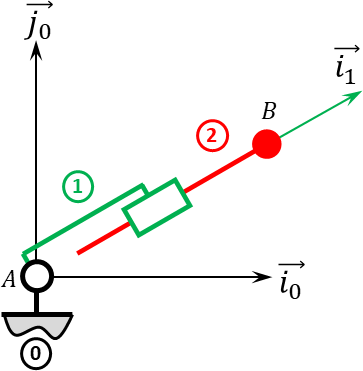
\includegraphics[width=\linewidth]{05_RT_01}
\end{center}
\fi

\question{Donner l'ensemble des positions accessibles par le point $B$.}
\ifprof
\else
\fi

\question{Donner l'équation horaire (trajectoire en fonction du temps) du point $B$ dans le mouvement de \textbf{2} par rapport à \textbf{0}.}
\ifprof
\else
\fi

On souhaite que le point $B$ réalise un segment entre les points $[-25,25]$ et $[25,25]$. 

\question{Donner les expressions de $\theta(t)$ et $\lambda(t)$ permettant la réalisation de cette trajectoire à la vitesse $v=\SI{0,01}{m.s^{-1}}$.}
\ifprof
\else
\fi


\question{En utilisant Python, tracer $\theta(t)$, $\lambda(t)$ et la trajectoire générée.}
\ifprof
\else
\fi

\ifprof
\else
\begin{flushright}
\footnotesize{Corrigé  voir \ref{B2:13:05}.}
\end{flushright}%
\fi